\documentclass[11pt]{article}
\pdfminorversion=7
\usepackage[letterpaper,top=0.75in,bottom=0.8in,left=0.8in,right=0.8in]{geometry}
\usepackage{amsmath,amssymb,amsthm,mathtools}
\usepackage[T1]{fontenc}
\usepackage{mathptmx}
\usepackage{courier}
\usepackage{microtype}
\usepackage{booktabs,longtable,array,tabularx,multirow}
\usepackage{graphicx}
\usepackage{float}
\usepackage{caption}
\usepackage{subcaption}
\usepackage{enumitem}
\usepackage{pdflscape}
\usepackage{xurl}
\usepackage{listings}
\usepackage{xcolor}
\usepackage[hidelinks]{hyperref}
\hypersetup{pdftitle={Boundary Limited Observer Systems: Computational and Formal Supplement},pdfauthor={Christopher Ezernack}}
\usepackage[nameinlink,capitalise]{cleveref}
\pagestyle{plain}
\setlength{\parindent}{0.25in}
\setlength{\parskip}{0pt}
\setlength{\emergencystretch}{2em}
\renewcommand{\arraystretch}{1.1}
\captionsetup{font=small,labelfont=bf,labelsep=period,justification=raggedright,singlelinecheck=false}
\setlist{nosep,leftmargin=2em}
\newcommand{\RepoCommit}{\texttt{eb96b984ae999ee6cbc0aae33c2d501c46d9540f}}
\lstdefinelanguage{Python}{
  morekeywords={def,return,for,in,if,not,and,True,False,class,property},
  sensitive=true,
  morecomment=[l]{\#},
  morestring=[b]",
  morestring=[b]'
}
\lstset{
  language=Python,
  basicstyle=\ttfamily\small,
  keywordstyle=\bfseries,
  commentstyle=\itshape,
  columns=fullflexible,
  keepspaces=true,
  frame=single,
  framerule=0.35pt,
  rulecolor=\color{black!45},
  backgroundcolor=\color{black!2},
  breaklines=true,
  showstringspaces=false
}
\begin{document}
\begin{flushleft}
{\LARGE\bfseries Boundary Limited Observer Systems}\par
\vspace{0.25em}
{\large Computational and Formal Supplement}\par
\vspace{0.5em}
{\normalsize Christopher Ezernack}\par
\end{flushleft}
\vspace{0.5em}
\hrule
\vspace{0.8em}

The finite model assigns hidden labels to each source state and records only the base coordinate. The code enumerates states with identical readings, calculates the possible results of each processing rule, and compares interfaces. The tables identify the corresponding Lean declarations (Appendix~\ref{app:declarations}), finite counts (Appendix~\ref{app:fulldata}), and source files (Appendix~\ref{app:provenance}).

\section{Executable implementation excerpts}

The following excerpts are copied from the repository implementation at commit \nolinkurl{eb96b984ae999ee6cbc0aae33c2d501c46d9540f}. They are included to show the executable operations underlying the finite summaries. The complete source remains in the repository.

\subsection{Collision count}
\begin{lstlisting}[language=Python]
@property
def latent_collision_count(self) -> int:
    return sum(
        comb(len(fiber), 2)
        for fiber in self.observation_fibers().values()
    )
\end{lstlisting}

\subsection{Finite hidden extension}
\begin{lstlisting}[language=Python]
latent_states = tuple(
    (state, hidden)
    for state in base.latent_states
    for hidden in range(multiplicity)
)
observation_by_state = {
    state: base.observe(state[0])
    for state in latent_states
}
\end{lstlisting}

\subsection{Observation only outcomes}
\begin{lstlisting}[language=Python]
def possible_outcomes(self, model):
    return frozenset(
        self.transform(observation)
        for observation in model.reachable_observations
    )
\end{lstlisting}

\subsection{Finite empirical quotient grouping}
\begin{lstlisting}[language=Python]
grouped = {}
for model in models:
    grouped.setdefault(
        model.reachable_observations, []
    ).append(model)
\end{lstlisting}

\subsection{Collapsed pairs under coarsening}
\begin{lstlisting}[language=Python]
return tuple(
    (left, right)
    for left, right in combinations(
        self.fine.world_states, 2
    )
    if not self.fine.observationally_equivalent(left, right)
    and self.coarse.observationally_equivalent(left, right)
)
\end{lstlisting}

\appendix
\begin{landscape}
\section{Lean declarations}
\label{app:declarations}

Table~\ref{tab:declarations} identifies the declarations in \nolinkurl{BoundaryObserver.lean} for each mathematical result.

\small
\begin{longtable}{@{}>{\raggedright\arraybackslash}p{0.31\linewidth}>{\raggedright\arraybackslash}p{0.20\linewidth}>{\raggedright\arraybackslash}p{0.41\linewidth}@{}}
\caption{Definitions and theorems in Lean}\label{tab:declarations}\\
\toprule
Declaration & Paper section & Verified role \\
\midrule
\endfirsthead
\toprule
Declaration & Paper section & Verified role \\
\midrule
\endhead
\bottomrule
\endfoot
\nolinkurl{ObserverInterface} & Article, Appendix B & Declares an observation type and a map from world states to observations. \\
\nolinkurl{ObsEq} & Article, Appendix B & Defines state equivalence by equality of accessible observations. \\
\nolinkurl{factorized_quantity_respects_obsEq} & Article, Appendix B & Proves that interface factorized quantities are constant on observation fibers. \\
\nolinkurl{exact_decoder_implies_injective} & Article, Appendix B & Proves that a globally exact decoder implies observation injectivity. \\
\nolinkurl{no_exact_decoder_of_not_injective} & Article, Appendix B & Gives the reconstruction obstruction for a noninjective map. \\
\nolinkurl{internal_test_cannot_distinguish_obsEq} & Article, Appendix B & Proves that an observation only binary test cannot separate one fiber. \\
\nolinkurl{finite_interface_has_collision} & Article, Appendix B & Uses finite cardinality to produce distinct states with one observation. \\
\nolinkurl{finite_interface_has_no_exact_decoder} & Article, Appendix B & Connects finite capacity deficit to exact decoder failure. \\
\nolinkurl{ObservableQuotient} & Article, Appendix C & Quotients world states by observational equivalence. \\
\nolinkurl{observableQuotient_universal_property} & Article, Appendix C & Characterizes unique factorization of fiber constant quantities. \\
\nolinkurl{observable_variation_prevents_factorization} & Article, Appendix C & Shows that variation within one fiber prevents interface factorization. \\
\nolinkurl{InterfaceRefines} & Article, Appendix D & Defines coarsening by a commuting observation equation. \\
\nolinkurl{refinement_preserves_obsEq} & Article, Appendix D & Proves that fine equivalence implies coarse equivalence. \\
\nolinkurl{factorization_monotone_under_refinement} & Article, Appendix D & Lifts every coarse accessible quantity to the fine interface. \\
\nolinkurl{quotientMapOfRefinement_surjective} & Article, Appendix D & Proves that the induced fine to coarse quotient map is surjective. \\
\nolinkurl{strictlyRefines_prevents_reverse_refinement} & Article, Appendix D & Proves that strict refinement cannot be reversed. \\
\nolinkurl{strictlyRefines_quotientMap_not_injective} & Article, Appendix D & Proves that strict coarsening collapses quotient classes. \\
\nolinkurl{quotientMapOfMutualRefinement_bijective} & Article, Appendix D & Establishes quotient bijection under mutual refinement. \\
\nolinkurl{GenerativeModel} & Article, Appendix E & Declares a latent state type and a latent to observation map. \\
\nolinkurl{Produces} & Article, Appendix E & Defines reachability of one observation. \\
\nolinkurl{ModelObsEq} & Article, Appendix E & Defines model equivalence by equality of produced observations. \\
\nolinkurl{ExperimentOutcomeSet} & Article, Appendix E & Collects the possible results of one admissible experiment. \\
\nolinkurl{modelObsEq_preserves_experimentOutcomeSet} & Article, Appendix E & Proves outcome set equality for empirically equivalent models. \\
\nolinkurl{identityExperiment} & Article, Appendix E & Returns the accessible observation unchanged. \\
\nolinkurl{exactLatentDecoder_not_determinedBy_identityExperiment} & Article, Appendix F & Proves that even complete accessible observations do not determine decoder existence. \\
\nolinkurl{PredicateProfile} & Article, Appendix F & Records which accessible predicates can succeed. \\
\nolinkurl{modelObsEq_iff_predicateProfile_eq} & Article, Appendix F & Characterizes empirical equivalence by complete predicate profiles. \\
\nolinkurl{exactLatentDecoder_not_determinedByPredicateProfile} & Article, Appendix F & Shows that complete predicate profiles do not determine exact reconstruction. \\
\nolinkurl{LatentCover} & Article, Appendix G & Declares a surjective observation preserving projection to a base model. \\
\nolinkurl{StrictLatentCover} & Article, Appendix G & Adds noninjectivity of the latent projection. \\
\nolinkurl{hiddenExtensionModel} & Article, Appendix G & Adjoins a hidden factor and ignores it during observation. \\
\nolinkurl{finiteMultiplicityModel} & Article, Appendix G & Creates arbitrary finite hidden multiplicity. \\
\nolinkurl{countableMultiplicityModel} & Article, Appendix G & Creates a natural number hidden coordinate. \\
\nolinkurl{countableMultiplicityFiber_contains_nat} & Article, Appendix G & Embeds the natural numbers into one observation fiber. \\
\nolinkurl{no_inhabited_model_is_latentlyMaximal} & Article, Appendix G & Constructs a strict empirically equivalent extension of every inhabited model. \\
\nolinkurl{EmpiricalModelQuotient} & Article, Appendix H & Quotients generative models by empirical equivalence. \\
\nolinkurl{observationInvariant_iff_factorsThroughEmpiricalModelQuotient} & Article, Appendix H & Characterizes observation invariant properties by quotient factorization. \\
\nolinkurl{empiricalModelQuotient_map_universal_property} & Article, Appendix H & Gives unique descent of arbitrary observation invariant measurements. \\
\nolinkurl{exactLatentDecoder_not_factorsThroughEmpiricalModelQuotient} & Article, Appendix H & Proves that decoder existence is not a property of the empirical class. \\
\nolinkurl{empiricalModelQuotientEquivRealizableObservationSet} & Article, Appendix H & Identifies empirical classes with realizable reachable observation sets. \\
\nolinkurl{boundaryLimitedObserver_synthesis} & Article, Appendix I & Constructs the strict Boolean extension with the five conclusions of the synthesis theorem. \\
\end{longtable}
\end{landscape}

\begin{landscape}
\section{Finite model data}
\label{app:fulldata}

The files in \nolinkurl{data/original_csv/} contain the complete finite calculations. The tables report the values in these files.

\subsection{Complete model summary}

\scriptsize
\begin{longtable}{@{}lrrrrrrccc@{}}
\caption{Complete \texttt{model\_summary.csv}}\label{tab:fullmodelsummary}\\
\toprule
Model & Latent & Reachable & Avg fiber & Max fiber & Collisions & Multiplicity & Injective & Decoder & Hidden kind \\
\midrule
\endfirsthead
\toprule
Model & Latent & Reachable & Avg fiber & Max fiber & Collisions & Multiplicity & Injective & Decoder & Hidden kind \\
\midrule
\endhead
injective\_base & 6 & 6 & 1.00 & 1 & 0 & 1 & True & True & none \\
noninjective\_base & 6 & 3 & 2.00 & 2 & 3 & 1 & False & False & none \\
boolean\_hidden\_extension & 12 & 6 & 2.00 & 2 & 6 & 2 & False & False & boolean \\
injective\_base\_1\_fold\_extension & 6 & 6 & 1.00 & 1 & 0 & 1 & True & True & finite \\
injective\_base\_2\_fold\_extension & 12 & 6 & 2.00 & 2 & 6 & 2 & False & False & finite \\
injective\_base\_3\_fold\_extension & 18 & 6 & 3.00 & 3 & 18 & 3 & False & False & finite \\
injective\_base\_5\_fold\_extension & 30 & 6 & 5.00 & 5 & 60 & 5 & False & False & finite \\
injective\_base\_8\_fold\_extension & 48 & 6 & 8.00 & 8 & 168 & 8 & False & False & finite \\
\bottomrule
\end{longtable}
\end{landscape}

\begin{landscape}
\subsection{Complete experiment outcome records}
\scriptsize
\begin{longtable}{@{}p{0.13\linewidth}p{0.27\linewidth}rp{0.25\linewidth}rc@{}}
\caption{Complete \texttt{experiment\_outcomes.csv}}\label{tab:fullexperiments}\\
\toprule
Experiment & Model & Multiplicity & Possible outcomes & Count & Matches base \\
\midrule
\endfirsthead
\toprule
Experiment & Model & Multiplicity & Possible outcomes & Count & Matches base \\
\midrule
\endhead
identity & injective\_base & 1 & \{0, 1, 2, 3, 4, 5\} & 6 & True \\
identity & boolean\_hidden\_extension & 2 & \{0, 1, 2, 3, 4, 5\} & 6 & True \\
identity & injective\_base\_1\_fold\_extension & 1 & \{0, 1, 2, 3, 4, 5\} & 6 & True \\
identity & injective\_base\_2\_fold\_extension & 2 & \{0, 1, 2, 3, 4, 5\} & 6 & True \\
identity & injective\_base\_3\_fold\_extension & 3 & \{0, 1, 2, 3, 4, 5\} & 6 & True \\
identity & injective\_base\_5\_fold\_extension & 5 & \{0, 1, 2, 3, 4, 5\} & 6 & True \\
identity & injective\_base\_8\_fold\_extension & 8 & \{0, 1, 2, 3, 4, 5\} & 6 & True \\
threshold\_at\_3 & injective\_base & 1 & \{False, True\} & 2 & True \\
threshold\_at\_3 & boolean\_hidden\_extension & 2 & \{False, True\} & 2 & True \\
threshold\_at\_3 & injective\_base\_1\_fold\_extension & 1 & \{False, True\} & 2 & True \\
threshold\_at\_3 & injective\_base\_2\_fold\_extension & 2 & \{False, True\} & 2 & True \\
threshold\_at\_3 & injective\_base\_3\_fold\_extension & 3 & \{False, True\} & 2 & True \\
threshold\_at\_3 & injective\_base\_5\_fold\_extension & 5 & \{False, True\} & 2 & True \\
threshold\_at\_3 & injective\_base\_8\_fold\_extension & 8 & \{False, True\} & 2 & True \\
categorical\_partition & injective\_base & 1 & \{'high', 'low', 'middle'\} & 3 & True \\
categorical\_partition & boolean\_hidden\_extension & 2 & \{'high', 'low', 'middle'\} & 3 & True \\
categorical\_partition & injective\_base\_1\_fold\_extension & 1 & \{'high', 'low', 'middle'\} & 3 & True \\
categorical\_partition & injective\_base\_2\_fold\_extension & 2 & \{'high', 'low', 'middle'\} & 3 & True \\
categorical\_partition & injective\_base\_3\_fold\_extension & 3 & \{'high', 'low', 'middle'\} & 3 & True \\
categorical\_partition & injective\_base\_5\_fold\_extension & 5 & \{'high', 'low', 'middle'\} & 3 & True \\
categorical\_partition & injective\_base\_8\_fold\_extension & 8 & \{'high', 'low', 'middle'\} & 3 & True \\
compressed\_width\_2 & injective\_base & 1 & \{0, 1, 2\} & 3 & True \\
compressed\_width\_2 & boolean\_hidden\_extension & 2 & \{0, 1, 2\} & 3 & True \\
compressed\_width\_2 & injective\_base\_1\_fold\_extension & 1 & \{0, 1, 2\} & 3 & True \\
compressed\_width\_2 & injective\_base\_2\_fold\_extension & 2 & \{0, 1, 2\} & 3 & True \\
compressed\_width\_2 & injective\_base\_3\_fold\_extension & 3 & \{0, 1, 2\} & 3 & True \\
compressed\_width\_2 & injective\_base\_5\_fold\_extension & 5 & \{0, 1, 2\} & 3 & True \\
compressed\_width\_2 & injective\_base\_8\_fold\_extension & 8 & \{0, 1, 2\} & 3 & True \\
\bottomrule
\end{longtable}

\end{landscape}

\subsection{Predicate records}
Each of three predicates was evaluated on all seven models. The 21 success profiles and the 21 truth tables match those of the base. The table gives the three distinct truth tables.
\begin{table}[H]
\centering
\caption{Unique predicate truth tables from \texttt{predicate\_truth\_profiles.csv}}
\begin{tabularx}{\textwidth}{@{}lXcc@{}}
\toprule
Predicate & Truth table & Success in base & All seven models match \\
\midrule
is\_even & 0:True; 1:False; 2:True; 3:False; 4:True; 5:False & True & True \\
at\_least\_three & 0:False; 1:False; 2:False; 3:True; 4:True; 5:True & True & True \\
is\_endpoint & 0:True; 1:False; 2:False; 3:False; 4:False; 5:True & True & True \\
\bottomrule
\end{tabularx}
\end{table}

\subsection{Empirical quotient and varying properties}
\begin{table}[H]
\centering
\caption{Complete \texttt{empirical\_quotient.csv}}
\scriptsize
\begin{tabularx}{\textwidth}{@{}cXlXc@{}}
\toprule
Class & Reachable set & Latent cardinalities & Models & Multiple cardinalities \\
\midrule
1 & \{0, 1, 2, 3, 4, 5\} & 6; 12; 18; 30; 48 & injective\_base; boolean\_hidden\_extension; injective\_base\_1\_fold\_extension; injective\_base\_2\_fold\_extension; injective\_base\_3\_fold\_extension; injective\_base\_5\_fold\_extension; injective\_base\_8\_fold\_extension & True \\
2 & \{0, 1, 2\} & 6 & noninjective\_base & False \\
\bottomrule
\end{tabularx}
\end{table}

\begin{table}[H]
\centering
\caption{Complete \texttt{nonidentifiable\_properties.csv}}
\begin{tabularx}{\textwidth}{@{}Xccccc@{}}
\toprule
Property & Base & Extension & Varies & Reach equal & Outcomes equal \\
\midrule
latent cardinality & 6 & 12 & True & True & True \\
maximum observation fiber size & 1 & 2 & True & True & True \\
existence of an exact latent decoder & True & False & True & True & True \\
presence of a Boolean hidden factor & False & True & True & True & True \\
\bottomrule
\end{tabularx}
\end{table}

\subsection{Complete interface and refinement summaries}
\begin{table}[H]
\centering
\caption{Complete \texttt{interface\_summary.csv}}
\begin{tabularx}{\textwidth}{@{}lrrrXrc@{}}
\toprule
Interface & World & Codomain & Reachable & Reachable values & Quotient & Injective \\
\midrule
identity\_interface & 8 & 8 & 8 & \{0, 1, 2, 3, 4, 5, 6, 7\} & 8 & True \\
paired\_bucket\_interface & 8 & 4 & 4 & \{0, 1, 2, 3\} & 4 & False \\
binary\_region\_interface & 8 & 2 & 2 & \{'lower', 'upper'\} & 2 & False \\
relabeled\_identity\_interface & 8 & 8 & 8 & \{'state\_0', 'state\_1', 'state\_2', 'state\_3', 'state\_4', 'state\_5', 'state\_6', 'state\_7'\} & 8 & True \\
\bottomrule
\end{tabularx}
\end{table}

\begin{landscape}
\scriptsize
\begin{longtable}{@{}lllrrrrcccc@{}}
\caption{Selected complete fields from \texttt{refinement\_summary.csv}}\label{tab:fullrefinement}\\
\toprule
Refinement & Fine & Coarse & Fine Q & Coarse Q & Collapsed & Strict & Reverse & Surjective & Injective & Bijective \\
\midrule
\endfirsthead
\toprule
Refinement & Fine & Coarse & Fine Q & Coarse Q & Collapsed & Strict & Reverse & Surjective & Injective & Bijective \\
\midrule
\endhead
identity\_to\_paired & identity\_interface & paired\_bucket\_interface & 8 & 4 & 4 & True & False & True & False & False \\
paired\_to\_region & paired\_bucket\_interface & binary\_region\_interface & 4 & 2 & 8 & True & False & True & False & False \\
identity\_to\_region & identity\_interface & binary\_region\_interface & 8 & 2 & 12 & True & False & True & False & False \\
identity\_to\_relabeled & identity\_interface & relabeled\_identity\_interface & 8 & 8 & 0 & False & True & True & True & True \\
relabeled\_to\_identity & relabeled\_identity\_interface & identity\_interface & 8 & 8 & 0 & False & True & True & True & True \\
\bottomrule
\end{longtable}
\end{landscape}

The files \texttt{observation\_fibers.csv}, \texttt{quotient\_maps.csv}, and \texttt{collapsed\_pairs.csv} contain the unaggregated fiber, class map, and pair records. Each row identifies an individual fiber, class mapping, or pair.

\section{Finite model figures}
\label{app:originalfigures}

The six figures use the CSV data in \nolinkurl{data/original_csv/}. The original image files are in \nolinkurl{original_repo_pngs/}.

\begin{figure}[H]
\centering
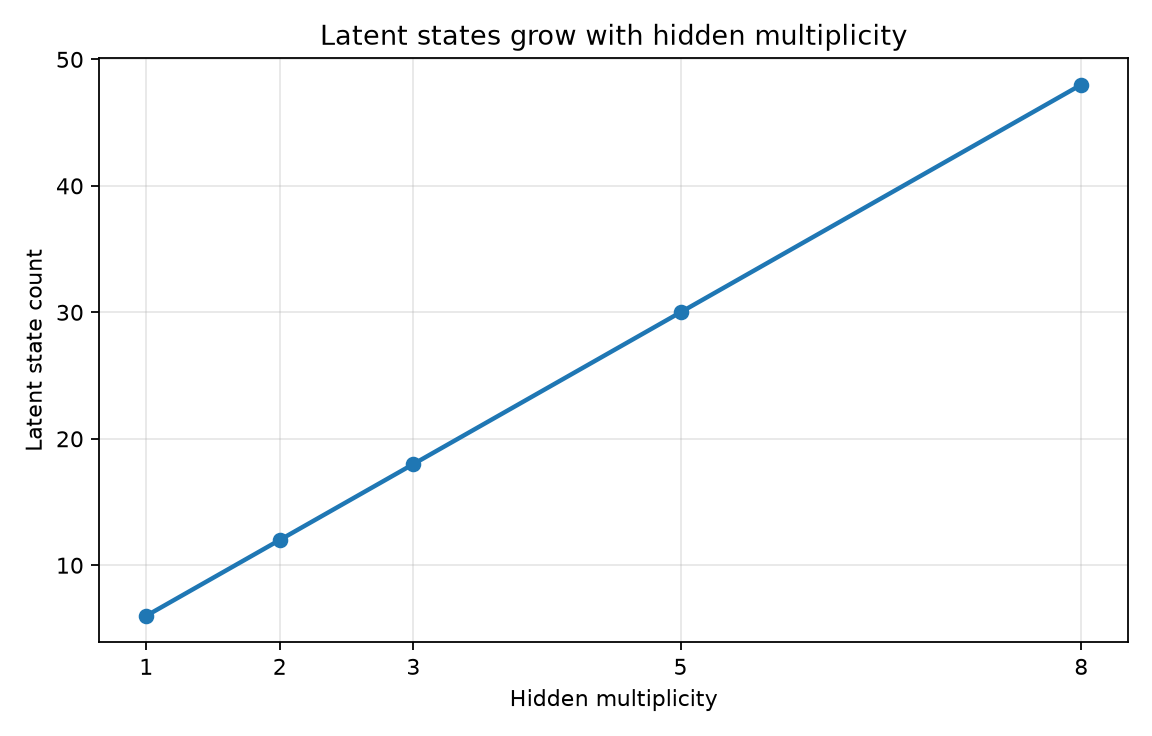
\includegraphics[width=0.86\textwidth]{original_repo_pngs/latent_state_count_vs_hidden_multiplicity.png}
\caption{Each hidden label adds six source states.}
\end{figure}

\begin{figure}[H]
\centering
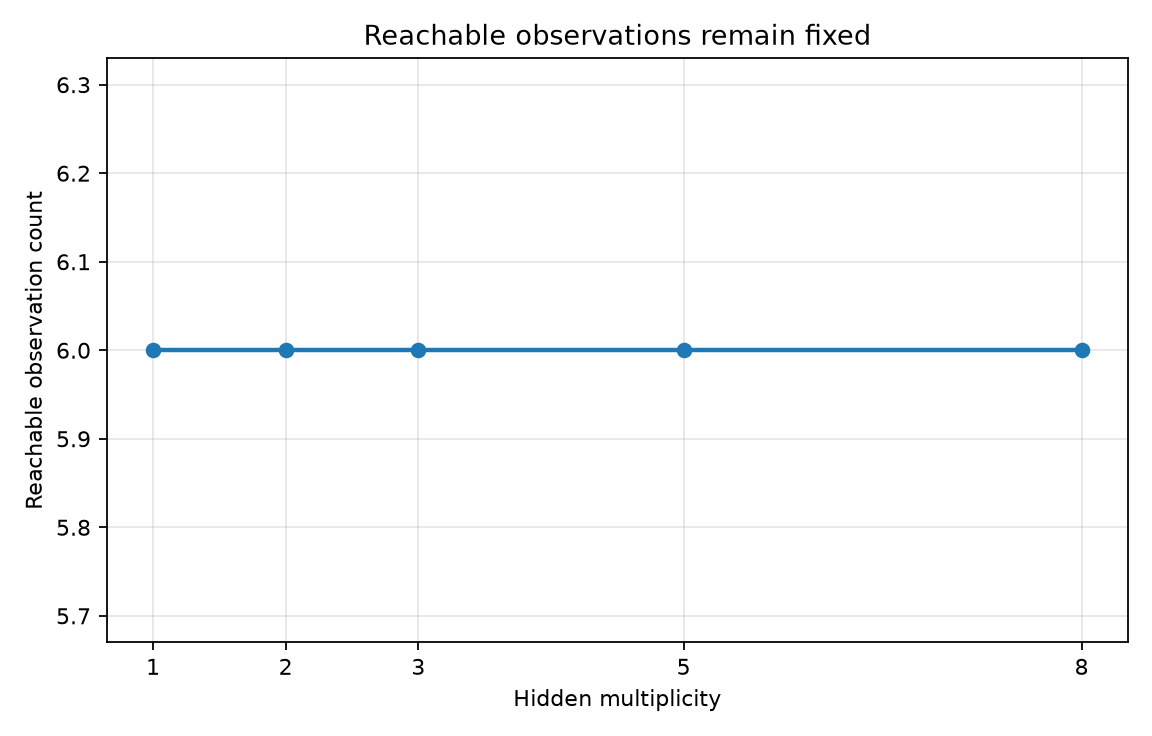
\includegraphics[width=0.86\textwidth]{original_repo_pngs/reachable_observation_count_vs_hidden_multiplicity.png}
\caption{The number of reachable observations stays at six as hidden multiplicity increases.}
\end{figure}

\begin{figure}[H]
\centering
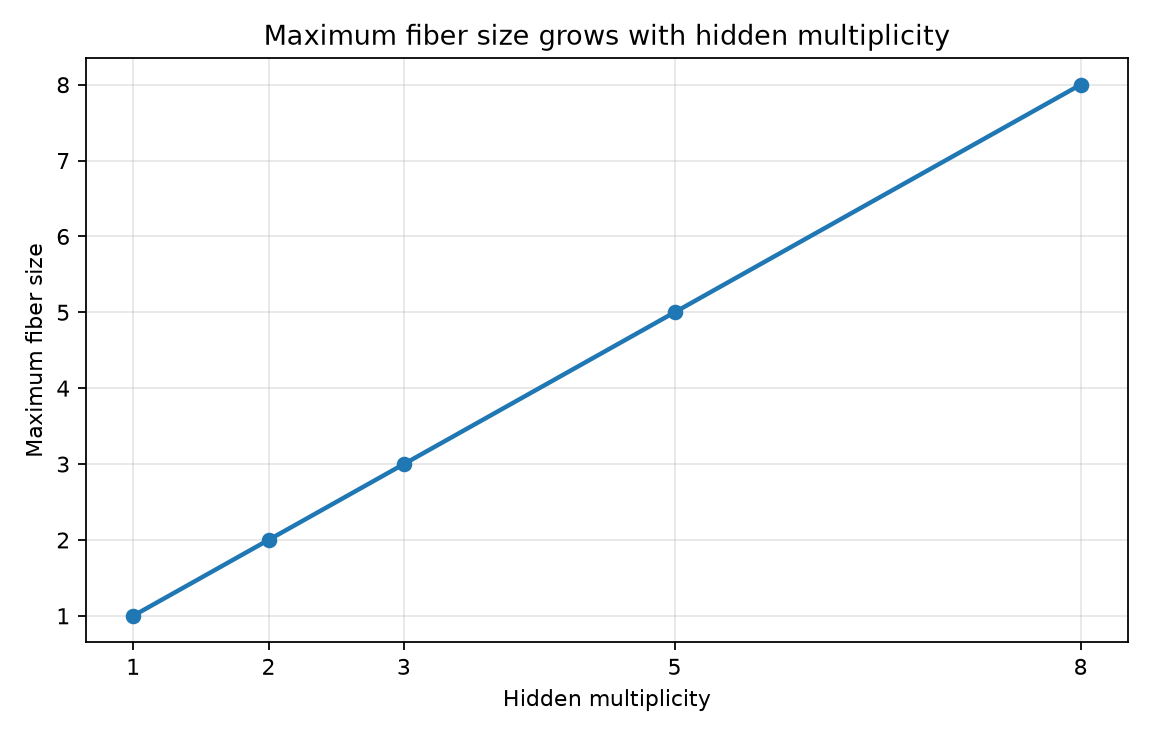
\includegraphics[width=0.86\textwidth]{original_repo_pngs/maximum_fiber_size_vs_hidden_multiplicity.png}
\caption{The maximum fiber size equals the number of hidden labels at each multiplicity.}
\end{figure}

\begin{figure}[H]
\centering
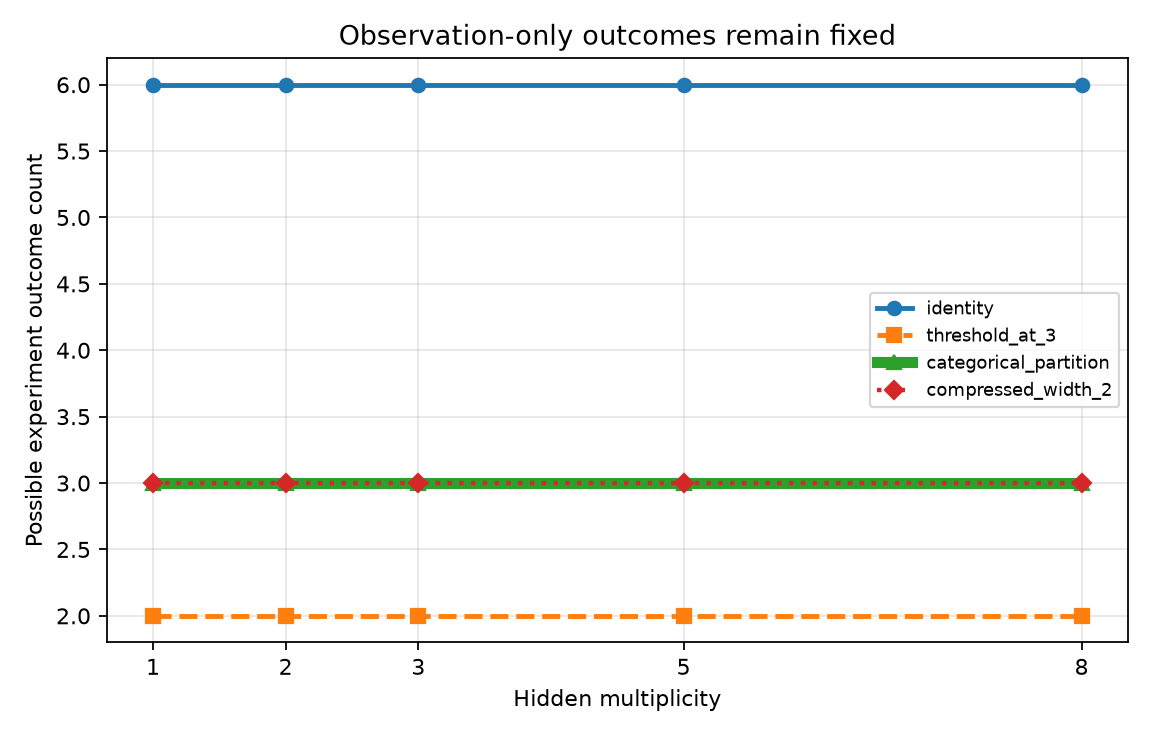
\includegraphics[width=0.86\textwidth]{original_repo_pngs/experiment_outcome_count_vs_hidden_multiplicity.png}
\caption{Each rule has a fixed number of possible outcomes across the six-output models.}
\end{figure}

\begin{figure}[H]
\centering
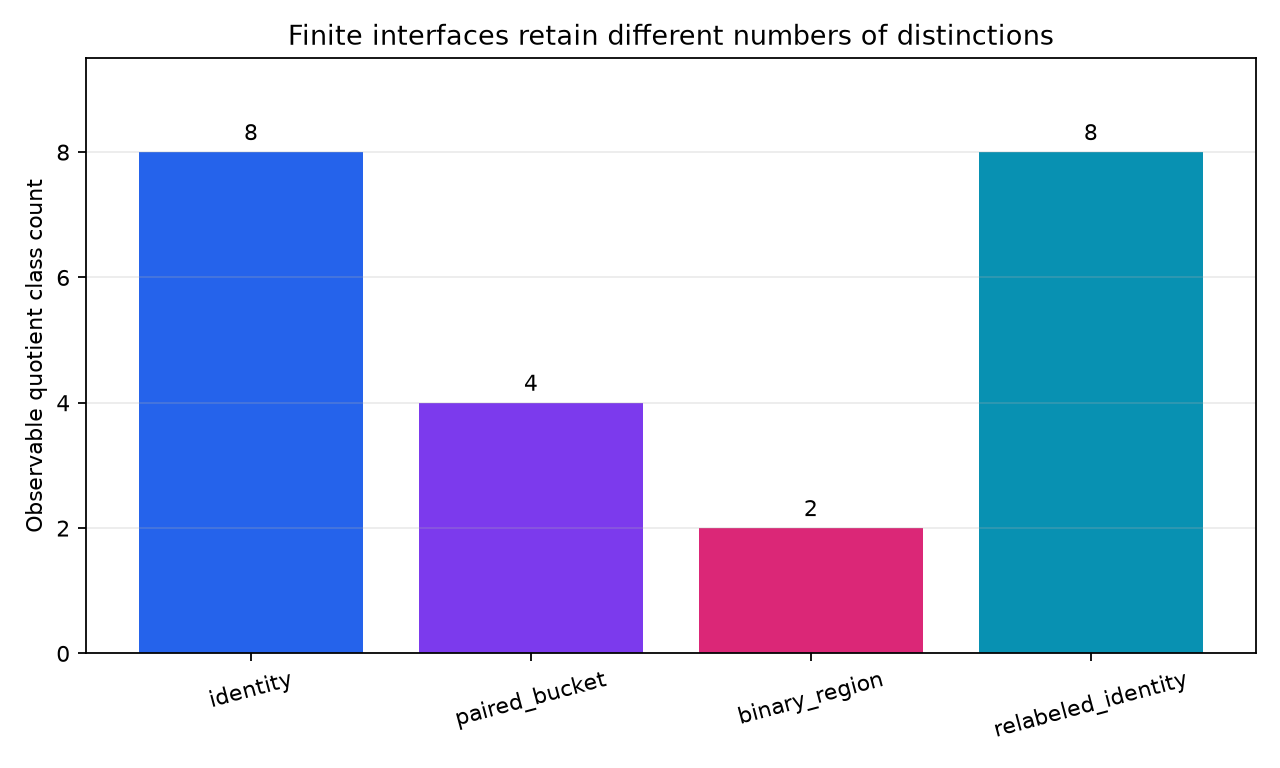
\includegraphics[width=0.90\textwidth]{original_repo_pngs/observable_quotient_size_by_interface.png}
\caption{Identity and relabeled identity retain eight classes. Paired buckets retain four and binary regions retain two.}
\end{figure}

\begin{figure}[H]
\centering
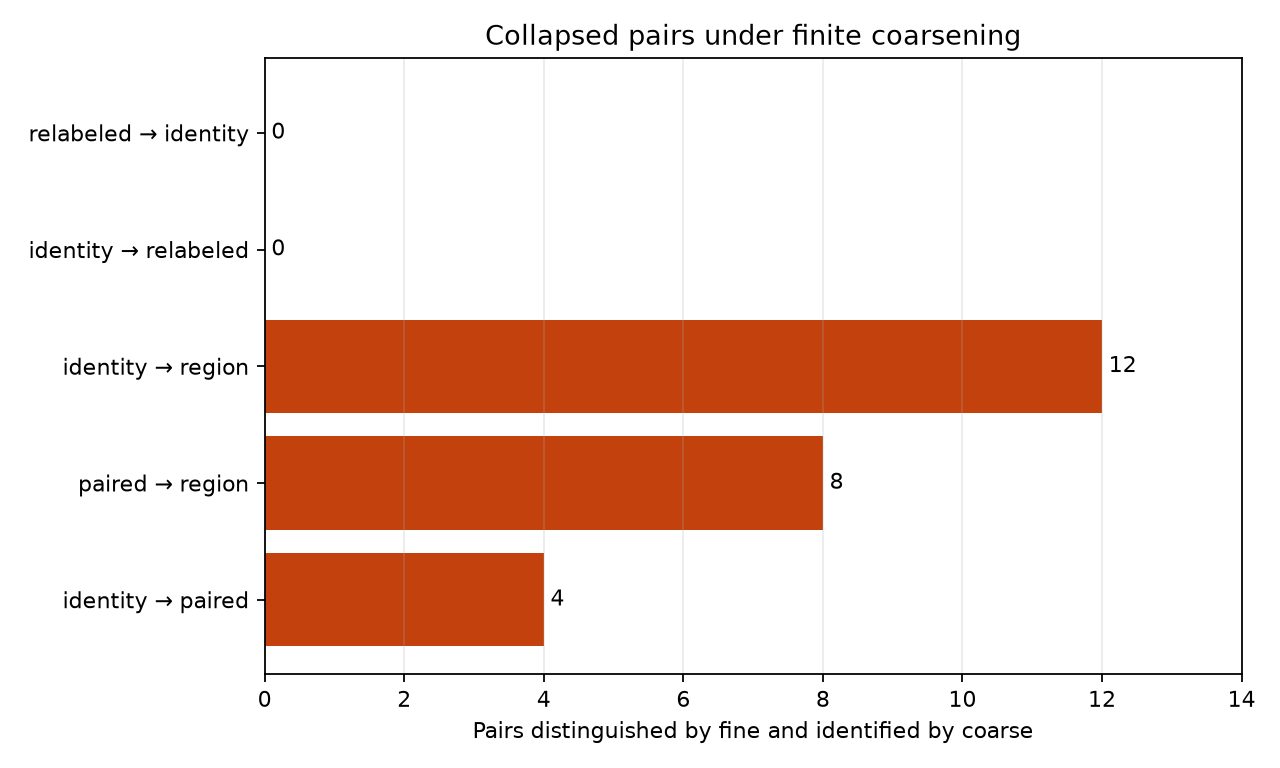
\includegraphics[width=0.90\textwidth]{original_repo_pngs/collapsed_pairs_by_refinement.png}
\caption{The three strict coarsenings merge four, eight, and twelve pairs, respectively. Relabeling merges none.}
\end{figure}

\section{Data provenance and file integrity}
\label{app:provenance}

The manifest was generated from the files included with this paper. Git blob hashes were calculated with \texttt{git hash-object}. SHA256 hashes were calculated from the file bytes. The full hashes are stored in \texttt{data\_manifest.json}; abbreviated Git blob hashes are printed below.

\begin{longtable}{@{}lrrl@{}}
\caption{Committed CSV provenance}\label{tab:manifest}\\
\toprule
File & Data rows & Git blob SHA prefix & Role \\
\midrule
\endfirsthead
\toprule
File & Data rows & Git blob SHA prefix & Role \\
\midrule
\endhead
collapsed\_pairs.csv & 24 & \texttt{fa8eff261917} & Unaggregated strict collapse records \\
empirical\_quotient.csv & 2 & \texttt{f3b32c8e14b1} & Finite empirical classes \\
experiment\_outcomes.csv & 28 & \texttt{7aab2b56cd54} & Possible outcome sets \\
interface\_summary.csv & 4 & \texttt{421487d5c9ce} & Finite interface summaries \\
model\_summary.csv & 8 & \texttt{754a77f53d49} & All finite model summaries \\
multiplicity\_summary.csv & 5 & \texttt{50b3754b844c} & Hidden multiplicity family \\
nonidentifiable\_properties.csv & 4 & \texttt{fb0af96c7411} & Latent property variation \\
observation\_fibers.csv & 45 & \texttt{e7708885ecc8} & Unaggregated observation fibers \\
predicate\_success\_profiles.csv & 21 & \texttt{b01193699afb} & Existential predicate profiles \\
predicate\_truth\_profiles.csv & 21 & \texttt{bf36618ee015} & Complete finite truth profiles \\
quotient\_maps.csv & 36 & \texttt{498dacd13751} & Unaggregated quotient map entries \\
refinement\_summary.csv & 5 & \texttt{b9cfae935abf} & Refinement and quotient map summary \\
\bottomrule
\end{longtable}

The original repository PNG files are also hash recorded. The vector paper figures are generated products and are not represented as committed repository PNGs. The collision plot is explicitly marked supplemental because no collision PNG is produced by the current repository runner.

\subsection{Validation record}
\begin{table}[H]
\centering
\caption{Repository validation record used by the paper}
\begin{tabularx}{\textwidth}{@{}lX@{}}
\toprule
Check & Recorded result \\
\midrule
Local Lean compilation in this revision & Not rerun \\
Repository Lean CI & Successful for the pinned commit; \url{https://github.com/ezernackchristopher97-cloud/BoundaryObserver/actions/runs/29449488270} \\
Unfinished proof commands & None in project source \\
Simulation runner & Completed all Boolean, multiplicity, experiment, predicate, quotient, and refinement assertions \\
Automated tests & 18 repository tests and 6 revision regression tests passed \\
CSV reproduction & All 12 files byte identical to the archived outputs \\
Repository state & Commit \RepoCommit \\
\bottomrule
\end{tabularx}
\end{table}

\subsection{Reproduce the finite checks}
Run the following commands from the \nolinkurl{paper/} directory to check the finite models and compare all twelve CSV files.
\begin{lstlisting}[language={}]
python -m pytest verification/reference_code/simulations/tests \
  verification/test_scope_cases.py verification/test_round_two.py -q
python verification/verify_outputs.py
\end{lstlisting}
The two tests in \nolinkurl{test_round_two.py} enumerate small reachable sets and pairs of binary measurements.
\end{document}
